%%%%%%%%%%%%%%%%%%%%%%%%%%%%%%%%%%%%%%%%%%%%%%%%%%%%%%%%%%%%%%%%%%%%%
% PREAMBLE
%%%%%%%%%%%%%%%%%%%%%%%%%%%%%%%%%%%%%%%%%%%%%%%%%%%%%%%%%%%%%%%%%%%%%
%
% The following two commands will generate a PDF that follows all the requirements for submission
% and peer review.  Uncomment these commands to generate this output (and comment out the two lines below.)
%
% DOUBLE SPACE VERSION FOR SUBMISSION TO THE AMS
\documentclass[12pt]{article}
\usepackage{ametsoc}
\usepackage[pagewise]{lineno}
\linenumbers
%
% The following two commands will generate a single space, double column paper that closely
% matches an AMS journal page.  Uncomment these commands to generate this output (and comment
% out the two lines above. FOR AUTHOR USE ONLY. PAPERS SUBMITTED IN THIS FORMAT WILL BE RETURNED
% TO THE AUTHOR for submission with the correct formatting.
%
% TWO COLUMN JOURNAL PAGE LAYOUT FOR AUTHOR USE ONLY
%%%%\documentclass[10pt]{article}
%%%%\usepackage{ametsoc2col}
%
%%%%%%%%%%%%%%%%%%%%%%%%%%%%%%%%%%%%%%%%%%%%%%%%%%%%%%%%%%%%%%%%%%%%%
% ABSTRACT
%
% Enter your Abstract here
%%%%%%%%%%%%%%%%%%%%%%%%%%%%%%%%%%%%%%%%%%%%%%%%%%%%%%%%%%%%%%%%%%%%%
\newcommand{\myabstract}{
Direct measurements of rates of entrainment into and detrainment from cloud 
cores obtained from LES model cloud fields produce values twice as large as 
those produced from bulk conserved tracer budget calculations.  This difference 
can be explained by three effects: the presence of a shell of moist air around 
the cloud cores and drier air at the edge of the cloud core, correlations 
between entrainment rates and tracer values, and errors in the calculation of 
the bulk tracer budget.  Correlations between the vertical momentum and the 
entrainment rate create strong vertical momentum fluxes into the cloud core,
making the assumption that clouds entrain fluid with zero vertical momentum
incorrect.  Variability in the properties of the moist cloud shell has strong
impacts on entrainment values inferred from bulk tracer calculations.  These
results indicate the dynamics of the cloud shell should be included in 
parametrization of cumulus clouds used in general circulation models.
}
%
\begin{document}
%
%%%%%%%%%%%%%%%%%%%%%%%%%%%%%%%%%%%%%%%%%%%%%%%%%%%%%%%%%%%%%%%%%%%%%
% TITLE
%
% Enter your TITLE here
%%%%%%%%%%%%%%%%%%%%%%%%%%%%%%%%%%%%%%%%%%%%%%%%%%%%%%%%%%%%%%%%%%%%%
\title{\textbf{\large{The influence of the cloud shell on bulk tracer 
measurements of LES cloud entrainment}}}
%
% Author names, with corresponding author information. 
% [Update and move the \thanks{...} block as appropriate.]
%
\author{\textsc{Jordan T Dawe}
				\thanks{\textit{Corresponding author address:} 
				Jordan T Dawe, Department of Earth and Ocean Sciences, 
                                University of British Columbia, 6339 Stores Road,
                                Vancouver, BC, V6T 1Z4, Canada.
				\newline{E-mail: jdawe@eos.ubc.ca}}\quad\textsc{and Philip H Austin}\\
\textit{\footnotesize{Department of Earth and Ocean Sciences, University of 
                      British Columbia, Vancouver, BC, Canada.}}
}
%
% Formatting done here...Authors should skip over this.  See above for abstract.
\ifthenelse{\boolean{dc}}
{
\twocolumn[
\begin{@twocolumnfalse}
\amstitle

% Start Abstract (Enter your Abstract above.  Do not enter any text here)
\begin{center}
\begin{minipage}{13.0cm}
\begin{abstract}
	\myabstract
	\newline
	\begin{center}
		\rule{38mm}{0.2mm}
	\end{center}
\end{abstract}
\end{minipage}
\end{center}
\end{@twocolumnfalse}
]
}
{
\amstitle
\begin{abstract}
\myabstract
\end{abstract}
}
%%%%%%%%%%%%%%%%%%%%%%%%%%%%%%%%%%%%%%%%%%%%%%%%%%%%%%%%%%%%%%%%%%%%%
% MAIN BODY OF PAPER
%%%%%%%%%%%%%%%%%%%%%%%%%%%%%%%%%%%%%%%%%%%%%%%%%%%%%%%%%%%%%%%%%%%%%
\section{Introduction}

The rate at which air is entrained into and detrained from cumulus clouds 
affects cloud properties, cloud top height, and vertical transports of heat 
and moisture.  Proper simulation of these sub-grid scale effects in General 
Circulation Models (GCM) depends on the accurate parametrization of 
entrainment of environmental tracer properties into the clouds and detrainment 
of cloud properties into the environment 
\citep{Bechtold2008, De_Rooy2010}.  

Entrainment and detrainment rates impact GCM parametrization in several ways.
First, profiles of cloud vertical mass flux are usually calculated from 
parametrized entrainment values using the continuity equation for a 
simple entraining plume:
\begin{equation}
   \label{eq:continuity}
   \rho \frac{\partial a}{\partial t} 
   + \frac{\partial M_{core}}{\partial z} = E - D.
\end{equation}
Here $\rho$ is the
density of the air in kg m$^{-3}$; $a$ is the fractional cloud core area
(where cloud core is defined as
regions having condensed liquid water, positive buoyancy, and upward vertical
velocity); $M_{core}$ is vertical cloud core
mass flux (kg m$^{-2}$ s$^{-1}$) and $E$ and $D$ are mass entrainment
and detrainment rates (kg m$^{-3}$ s$^{-1}$). 

The point where the mass flux profile goes to zero then defines the location 
of cloud top.  This mass flux profile is combined with the entrainment rate 
of environmental air into the cloud to generate vertical profiles of cloud
moisture and temperature, and these profiles are then used to calculate the
moistening of the environment by detrainment of cloud fluid 
\citep{Tiedtke1989, Kain1990}.  Precipitation rates are also generated from the
mass flux and tracer profiles produced from the entrainment and detrainment
profiles.  The wide range of effects that the entrainment and detrainment have
make entrainment rate one of the strongest controls on the climate sensitivity 
of GCMs \citep{Stainforth2005, Rougier2009}.

Large Eddy Simulation (LES) is the primary tool used to study cloud entrainment
and detrainment rates.  LES mass entrainment and detrainment rates are typically
calculated using budgets of bulk conserved tracer variables to infer the amount
of fluid exchange between the clouds and the surrounding air.  
\cite{Siebesma1995} derive the following equations for entrainment and
detrainment of mass from a cloud core plume:
\begin{subequations}
  \label{eq:siebesmaED}
\begin{equation}
  \label{eq:siebesma_entrainment}
    E_{\phi S}(\phi_{core} - \phi_{env}) = - M_{core} \frac{\partial \phi_{core}}{\partial z}
        - \frac{\partial \rho a \overline{w' \phi'}^{core}}{\partial z}
        - \rho a \frac{\partial \phi_{core}}{\partial t}
        + a \rho \left(\frac{\partial \bar{\phi}}{\partial t}\right)_{forcing}
\end{equation}
and
\begin{equation}
  \label{eq:siebesma_detrainment}
    D_{\phi S}(\phi_{core} - \phi_{env}) = - M_{core} \frac{\partial \phi_{env}}{\partial z}
        + \frac{\partial \rho (1 - a) \overline{w' \phi'}^{env}}{\partial z}
        + \rho (1-a) \frac{\partial \phi_{env}}{\partial t}
     - \rho (1-a) \left(\frac{\partial \bar{\phi}}{\partial t}\right)_{forcing}
\end{equation}
\end{subequations}
Where $\phi$ (with units denoted by $[\phi]$) represents any conserved
bulk tracer, such as the total specific humidity $q_t$ (kg water
kg$^{-1}$ moist air) or the liquid-water moist static energy $h$ (J
kg$^{-1}$); $w$ is vertical velocity (m
s$^{-1}$); $env$ and $core$ sub-and super-scripts denote horizontally
averaged values conditionally sampled in the cloud environment and
core; $forcing$ refers to tracer sources and sinks, such as radiation
or subsidence, not included in the other terms; primed values
represent anomalies relative to the horizontal mean; overbars
represent horizontal averaging; and $E_{\phi S}(z)$ and $D_{\phi
  S}(z)$ are the total mass entrainment into and detrainment from the
cloud core inferred from the bulk tracer budget, in kg s$^{-1}$
m$^{-3}$.  We use the $S$ subscript to differentiate $E$ and $D$
calculated via the Siebesma bulk tracer budget method from other
measures of mass exchanges, and we shall refer to values calculated by
this method as ``Siebesma tracer budget" entrainment and detrainment.
For convenience, the various tracer and entrainment/detrainment rate subscripts 
used below are summarized in the Appendix.

Alternatively, entrainment and detrainment of mass can be calculated directly
from the LES velocity and tracer fields.  \cite{Romps2010} recently presented a 
technique to measure local (grid scale) mass entrainment $e(x,y,z)$ and
detrainment $d(x,y,z)$.  Summing these point measurements horizontally gives 
$E_d(z)$ and $D_d(z)$, the total mass entrained into and detrained from the
cloud core field in kg s$^{-1}$ m$^{-3}$, where the $d$ subscript indicates 
these quantities were calculated directly from the model velocity and tracer
fields.  His equation (2) is:
\begin{equation}
  \label{eq:romps_e_minus_d}
  e - d = \frac{\partial}{\partial t}(\mathcal{A}\rho) 
        + \nabla \cdot (\rho \mathbf{u} \mathcal{A}) 
\end{equation}
Here $\mathcal{A}$ is the ``activity'' of the fluid, where
$\mathcal{A}$ is one at cloud core points and zero otherwise, and
$\mathbf{u}$ is the velocity of the air in m s$^{-1}$.  The values of
$e - d$ are averaged over the time that a grid cell experiences mass
fluxes between an active and an inactive point, then positive $e-d$
values are considered to be purely $e$, and negative values, $d$.  As
noted above, we shall refer to entrainment and detrainment values
calculated by this method as ``direct" $E$ and $D$ and denote them
with the subscript $d$.

Romps found that direct calculation of the entrainment and
detrainment mass fluxes produced values roughly twice as large as
the Siebesma tracer budget calculations.  Romps attributed this difference
to the Siebesma tracer budget calculation assumption that fluid
exchanged between clouds and environment has the mean properties of
the cloud or environment, respectively.  Recent studies of the dense,
descending shell of moist air that forms around trade-wind cumulus
clouds \citep{Heus2008, Wang2010} suggest that the cloud shell
properties are quite different than the core or environment
properties, bolstering Romps' hypothesis.  Since fluid exchanges
between clouds and environment must pass through this shell, it is
likely that it plays an important role in entrainment and detrainment
dynamics.

Below we examine the sources of the discrepancy in entrainment and
detrainment values calculated via bulk tracer budgets and directly
from model fluxes.  We show that the discrepancy is explained by three
effects: the presence of the shell of moist air around the cloud cores
and drier air at the edge of the cloud core, correlations between
local entrainment rates and tracer values which enhance tracer fluxes
between the clouds and the environment, and errors in the calculation
of the bulk tracer budget.  We derive a relation to transform the
``direct" entrainment flux values into ``Siebesma tracer budget"
values suitable for use in one-dimensional simple entraining plume
cloud parametrizations, and then use these transformed fluxes to
evaluate the impact of the shell on bulk tracer entrainment and
detrainment rates of humidity and vertical velocity.  Finally, we
examine the dynamics that drives the strong correlations we find
between entrainment rate, humidity, and vertical velocity.

%===================================================

\section{Model description}

All LES calculations in this paper were made using the System for Atmospheric 
Modeling \citep[SAM;][]{Khairoutdinov2003}.  Two model runs were performed, 
configured as standard Global Energy and Water Cycle Experiment (GEWEX) 
Cloud System Studies \citep[GCSS;][]{Randall2003} experiments: a Barbados 
Oceanographic and Meteorological Experiment \citep[BOMEX;][]{Siebesma2003} run,
and an Atmospheric Radiation Measurement Study \citep[ARM;][]{Brown2002} run. 
The BOMEX run was performed on a 6.4 km x 6.4 km horizontal x 3.2 km vertical 
domain with 25 meter grid size in all directions for 6 hours, and the first 
three hours of simulation were discarded. The ARM run was performed on a 
7.68 km x 7.68 km x 4.5 km domain with 30 meter grid size.  Precipitation was 
disabled in both runs.

We have implemented the entrainment calculation scheme of \cite{Romps2010} in 
SAM, allowing us to calculate the mass of air entrained into and detrained from
cloud core directly from model $\rho$, $\mathbf{u}$, and $\mathcal{A}$.  
\citet[eq. 4]{Romps2010} also presents a method for calculating local 
entrainment and detrainment rates for any model bulk variable in the same
framework as (\ref{eq:romps_e_minus_d}), but neglects forcing and diffusion
terms.  These terms are significant for quantities like vertical momentum, so 
we modify Romps's equation to include their effects:
\begin{equation}
  \label{eq:romps_ephi_minus_dphi}
  e\phi - d\phi = \frac{\partial}{\partial t}(\phi \mathcal{A} \rho) 
                + \nabla \cdot (\phi \rho \mathbf{u} \mathcal{A})
                - \rho \mathcal{A}S_\phi
\end{equation}
where $S_\phi$ is any non-advective source or sink term for $\phi$, such as 
precipitation for $q_t$ or radiation for $h$, in units of $[\phi]$ s$^{-1}$.  

As with equation (\ref{eq:romps_e_minus_d}), the local $(e\phi)(x,y,z)$
and $(d\phi)(x,y,z)$ must be horizontally summed to give the total
tracer entrained into or detrained out of the cloud ensemble, but
since $\phi$ can be negative, it is possible for entrainment to reduce
and for detrainment to increase the quantity of tracer in the cloud
core.  To accommodate this effect, if the average value of $\phi$ is
positive over the time that a grid cell experiences mass fluxes
between an active and an inactive point, then positive $e\phi-d\phi$
values are considered to be purely $e\phi$, and negative
values, $d\phi$.  However, if the average of $\phi$ is
negative, then positive $e\phi-d\phi$ values are considered to be
purely $(d\phi)(x,y,z)$, and negative values, $(e\phi)(x,y,z)$.
Horizontal summation of $(e\phi)$ and $(d\phi)$ then gives
$(E\phi)_d(z)$ and $(D\phi)_d(z)$, the total entrainment and
detrainment of tracer for the cloud ensemble in units of $[\phi]$ kg s$^{-1}$
m$^{-3}$ calculated directly from the model velocity and tracer fields.

%===================================================

\section{Relationship Between Direct and Bulk Tracer Budget Entrainment}

\cite{Romps2010} established that the direct estimate of mass
entrainment and detrainment yields values roughly twice the size of
those calculated via bulk tracer budgets.  Furthermore, examination of
the ratios of the Siebesma tracer budget mass entrainment and detrainment
calculated via a total specific water budget ($E_qS$, $D_qS$) to the
directly calculated values ($E_d$, $D_d$) over the diurnal cycle of an
ARM LES reveals significant changes over the course of the day
(Fig.~\ref{fig:entrainment_ratio_variability}).  Thus the bulk tracer
and direct measurements of $E$ and $D$ are not only significantly
different, but have differing dynamics, which may need to be be accounted for
in large-scale parametrizations that account for entrainment and
detrainment.  In this section we examine the sources of disagreement
between direct and Siebesma tracer budget estimates of mass
entrainment into and detrainment from the cloud core. We first
consider the different assumptions about tracer values in the cloud
core and environment, then look at correlations between
entrainment/detrainment and tracer values and the different numerical
approximations made in the two budget calculations.

%---------------------------------------------------

\subsection{$E$ and $D$ Cloud Shell Correction}

Romps attributed the differences between ($E_{\phi S}$, $D_{\phi S}$)
and ($E_d$, $D_d$) to the assumption made by \cite{Siebesma1995} that
fluid entrained or detrained has the properties of the mean
environment or cloud core, respectively.  The fact that the mean core
and environment properties are not representative of entraining and
detraining fluid is shown in Fig. \ref{fig:Shell_correction}a. If we
examine the specific humidity of the fluid at the ``cloud core edge"
(cloud core model grid cells that are nearest-neighbor adjacent to
non-core cells), which presumably is the fluid being detrained, we see
it is drier than the mean core.  Similarly, the fluid just outside the
cloud core in the ``cloud core shell" (non-core model grid cells that
are nearest-neighbor adjacent to core cells) which is available for
entrainment is moister than the mean environment.

Budget equations that explicity distinguish between the the moist
cloud shell and dry cloud edge allow us to transform ($E_d, D_d$)
values into equivalent Siebesma tracer budget values ($E_{\phi S},
D_{\phi S}$) and back again.  We start our derivation by modifying
equations (5.1) from \cite{Siebesma1995}:
\begin{eqnarray}
  \label{eq:entrainment_derivation_1}
    \rho \frac{\partial a \phi_{core}}{\partial t} 
    = - \frac{\partial M_{core} \phi_{core}}{\partial z} 
    + E_d \phi_E - D_d \phi_D
    - \frac{\partial \rho a \overline{w' \phi'}^{core}}{\partial z} 
    + a \rho \left(\frac{\partial \bar{\phi}}{\partial t}\right)_{forcing}
\end{eqnarray}
\begin{eqnarray}
  \label{eq:detrainment_derivation_1}
    \rho \frac{\partial (1 - a) \phi_{env}}{\partial t}
    = \frac{\partial M_{core} \phi_{env}}{\partial z} 
    - E_d \phi_E + D_d \phi_D
    - \frac{\partial \rho (1 - a) \overline{w' \phi'}^{env}}{\partial z} 
    + \rho (1 - a) \left(\frac{\partial \bar{\phi}}{\partial t}\right)_{forcing}.
\end{eqnarray}
Here we have replaced $\phi_{env}$ in the entrainment term with $\phi_E$ and 
$\phi_{core}$ in the detrainment term with $\phi_D$, where $\phi_E$ and $\phi_D$
are the tracer values of the air being entrained and detrained, respectively.

Next we substitute equation (\ref{eq:continuity}), the continuity equation 
for a cloud plume, into (\ref{eq:entrainment_derivation_1}) 
and (\ref{eq:detrainment_derivation_1}) allowing us to write
\begin{eqnarray}
  \label{eq:entrainment_derivation_2}
    E_d (\phi_{core} - \phi_E) - D_d (\phi_{core} - \phi_D)
    = M_{core} \frac{\partial \phi_{core}}{\partial z}
    + \frac{\partial \rho a \overline{w' \phi'}^{core}}{\partial z} 
    + \rho a \frac{\partial \phi_{core}}{\partial t}
    - a \rho \left(\frac{\partial \bar{\phi}}{\partial t}\right)_{forcing}
\end{eqnarray}
\begin{eqnarray}
  \label{eq:detrainment_derivation_2}
    D_d (\phi_D - \phi_{env}) - E_d (\phi_E - \phi_{env})
    = - M_c \frac{\partial \phi_{env}}{\partial z}
    + \frac{\partial \rho (1 - a) \overline{w' \phi'}^{env}}{\partial z} 
    + \rho (1 - a) \frac{\partial \phi_{env}}{\partial t}
    - \rho (1 - a) \left(\frac{\partial \bar{\phi}}{\partial t}\right)_{forcing}.
\end{eqnarray}

We then substitute in (\ref{eq:siebesmaED})
for the bulk tracer tendency terms and 
rearrange to get:
\begin{subequations}
  \label{eq:correctedED}
\begin{equation}
  \label{eq:corrected_entrainment}
    E_{\phi T} = E_d 
             - \left[E_d\frac{(\phi_E - \phi_{env})}{(\phi_{core} - \phi_{env})}
                   + D_d\frac{(\phi_{core} - \phi_D)}{(\phi_{core} - \phi_{env})}\right]
\end{equation}
\begin{equation}
  \label{eq:corrected_detrainment}
    D_{\phi T} = D_d
             - \left[E_d\frac{(\phi_E - \phi_{env})}{(\phi_{core} - \phi_{env})}
                   + D_d\frac{(\phi_{core} - \phi_D)}{(\phi_{core} - \phi_{env})}\right].
\end{equation}
\end{subequations}
The bracketed terms represent the bias introduced by assuming that
entrained/detrained air has the propreties of the mean environment and
core.  Thus, to convert from ($E_d$,$D_d$) to ($E_{\phi T}$, $D_{\phi  T}$), 
both $E_d$ and $D_d$ must be reduced by $E_d A + D_d B$, where
$A = (\phi_E - \phi_{env})/(\phi_{core} - \phi_{env})$ and $B =
(\phi_{core} - \phi_D)/(\phi_{core} - \phi_{env})$.  Here we have
added the $T$ subscript to the $E_{\phi T}$ and $D_{\phi T}$ terms to
denote these values are equivalent to Siebesma tracer budget values,
but have been calculated by transforming the direct entrainment and
detrainment values.  We shall refer to these values as ``transformed"
entrainment and detrainment.

Alternatively, we can solve for $E_d$ and $D_d$, arriving at
\begin{subequations}
\begin{equation}
  \label{eq:corrected_entrainment2}
    E_{d T} = E_{\phi S} 
        + \left[E_{\phi S}\frac{(\phi_E - \phi_{env})}{(\phi_D - \phi_E)} 
              + D_{\phi S}\frac{(\phi_{core} - \phi_D)}{(\phi_D - \phi_E)}\right].
\end{equation}
\begin{equation}
  \label{eq:corrected_detrainment2}
    D_{d T} = D_{\phi S} 
        + \left[E_{\phi S}\frac{(\phi_E - \phi_{env})}{(\phi_D - \phi_E)}
              + D_{\phi S}\frac{(\phi_{core} - \phi_D)}{(\phi_D - \phi_E)}\right].
\end{equation}
\end{subequations}
In this case, to convert from ($E_{\phi S}$, $D_{\phi S}$) to
($E_{dT}$, $D_{dT}$), both $E_{\phi S}$ and $D_{\phi S}$ must be
increased by $E_{\phi S} a + D_{\phi S} b$, where $a = (\phi_E -
\phi_{env})/(\phi_{core} - \phi_{env})$ and $b = (\phi_{core} -
\phi_D)/(\phi_{core} - \phi_{env})$.  Note that under both these
transformations $E_d-D_d = E_{\phi}-D_{\phi}$, preserving mass
continuity, and furthermore, $E_d A + D_d B = E_{\phi} a + D_{\phi}
b$.

We now have relationships allowing us to transform the unbiased
$E_{d}$ and $D_{d}$ values into biased Siebesma tracer budget
$E_{\phi S}$ and $D_{\phi S}$ values, which are better suited for
simple entraining plume parametrization of cloud fields.
Comparison of $E_{q S}$ and $D_{q S}$ ($E_{\phi S}$ and $D_{\phi S}$ inferred
using total specific moisture $q_t$ as the bulk tracer) with $E_d$ and $D_d$
shows the direct entrainment and detrainment magnitudes are significantly larger 
than the Siebesma tracer budget values (Figure \ref{fig:Shell_correction}b 
and \ref{fig:Shell_correction}c, grey and dotted lines).  
Using  (\ref{eq:correctedED}) to calculate $E_{q T}$ and $D_{q T}$ with
$q_E = q_{edge}$ and $q_D = q_{shell}$ results in values quite close to 
the Siebesma tracer budget values above the middle of the cloud layer.   
The transformation also duplicates the negative 
detrainment values near cloud base that are typically produced by bulk tracer
calculations.

%-------------------------------------------------------------------------

\subsection{Entrainment/Tracer Correlations}

Relative to the Siebema tracer budget
values, the transformed $E_{q T}$ and $D_{q T}$ values are still too large 
near cloud base. 
We can partially explain the difference between the transformed mass 
entrainment/detrainment values and the Siebesma tracer budget values as 
being the result of correlations between the local entrainment/detrainment 
rates and the local tracer properties in the shell and edge.  Using the 
mean shell and edge values of tracers to transform the direct entrainment 
and detrainment assumes that any fluid parcel in the shell or edge is 
equally likely to be entrained or detrained.  In reality, mixing relatively 
dry air into the cloud core is more likely to cause evaporation, which will 
drive detrainment, while mixing relatively moist air into the cloud core is 
more likely to produce a saturated fluid mixture, resulting in entrainment.

If there are correlations between entrainment/detrainment and the local 
fluid properties, this will result in the effective tracer value 
entrained into or detrained from the cloud core being different than the 
mean tracer value in the shell or edge.  We can directly calculate the 
effective tracer value at which entrainment occurs by taking the total 
tracer entrainment $(E\phi)_d$ calculated via equation 
(\ref{eq:romps_ephi_minus_dphi}) and dividing it by the total mass
entrainment $E_d$ so that $\phi_{entrain} = (E\phi)_d / E_d$.  Similarly, 
the effective tracer value at which detrainment occurs can be found from  
$\phi_{detrain} = (D\phi)_d / D_d$.  Examination of these values from the 
BOMEX simulation using $q_t$ for $\phi$ shows $q_{entrain}$ is moister than 
$q_{shell}$ (Figure \ref{fig:Reynolds_correction}a), indicating entrainment
occurs preferentially at the moistest parts of the shell.  Conversely, 
there is little difference between between $q_{detrain}$ and $q_{edge}$,
indicating no significant correlation between detrainment and the moisture
present in the cloud core edge.

Using $q_{entrain}$ and $q_{detrain}$ to transform $E_d$ and $D_d$
results in smaller $E_{q T}$ and $D_{q T}$ values than utilizing the
mean shell and edge properties (solid black line,
Fig.~\ref{fig:Reynolds_correction}b and
\ref{fig:Reynolds_correction}c).  $E_{q T}$ calculated using $q_E =
q_{entrain}$ and $q_D = q_{detrain}$ is about half the magnitude of
the Siebesma tracer budget entrainment value throughout the cloud
layer.  This new transformation reduces the large entrainment and
detrainment values near cloud base, which improves the overall shape
of the fluxes. Above mid-cloud, howver, there is less correspondance 
between transformed $E_{q T}$ and $D_{q T}$ values and the Siebesma
tracer budget values $E_{q S}$ and $D_{q S}$ when compared to the 
shell and edge correction of Figure~\ref{fig:Reynolds_correction}.

%------------------------------------------------------------------------------

\subsection{Tracer Budget Errors}

The results above highlight the role of the definition of mean cloud
and environmental quantities in determining entrainment and detrainment
using tracer budgets.  An additional source for the discrepancy
between the bulk tracer budgets and their direct counterparts
is the  calculation of source and sink terms.
The Siebesma tracer budget calculated
using (\ref{eq:siebesmaED}) accounts for the
vertical advection of tracer properties by taking derivatives of mean 
vertical tracer profiles, along with averaged vertical Reynolds fluxes.  
There is no guarantee this estimate of vertical advection will exactly 
agree with the fully three dimensional MPDATA advection algorithm used by 
SAM.  In fact, the differences in the numerics of these calculations 
likely insures the results, while similar, will not be exactly the 
same.  Furthermore, the Siebesma calculation neglects tracer diffusion.  
These effects are likely small, but the exact amount of error they 
induce is difficult to evaluate.

\cite{Romps2010} presents an alternative to the Siebesma method of calculating 
bulk tracer budget entrainment and detrainment values (Romps' equations (11) 
and (12)) which uses the direct mass and $\phi$ entrainment/detrainment rates 
and mean profiles of $\phi_{core}$ and $\phi_{env}$ to calculate the vertical
advection and time tendency budgets (referred to as VATT below) 
that are on the right hand side of (\ref{eq:siebesmaED}):
\begin{subequations}
 \label{eq:romps_bulkED}
\begin{equation}
  \label{eq:romps_bulk_entrainment}
    E_{\phi R}(\phi_{core} - \phi_{env}) = \phi_{core}(E_d-D_d) - ((E\phi)_d - (D\phi)_d)
\end{equation}
\begin{equation}
  \label{eq:romps_bulk_detrainment}
    D_{\phi R}(\phi_{core} - \phi_{env}) = \phi_{env}(E_d-D_d) - ((E\phi)_d - (D\phi)_d)
\end{equation}
\end{subequations}
Here the $R$ subscript indicates that $E$ and $D$ have been calculated via 
the Romps bulk tracer budget method, and we shall refer to values calculated 
by this method as the  ``Romps tracer budget'' $E$ and $D$.

To see that the Romps tracer budget equations (\ref{eq:romps_bulkED}) account for exactly the same
source and sink terms as  the Siebesma 
tracer budget equations (\ref{eq:siebesmaED}),  first multipy  (\ref{eq:continuity})
by $\phi_{core}$:
\begin{equation}
    \phi_{core}(E_d - D_d) =
    \phi_{core} \left(\rho \frac{\partial a}{\partial t}
                    + \frac{\partial M_{core}}{\partial z}\right).
\end{equation}
If diffusion is neglected, the tracer continuity equation can be 
used to show that
\begin{equation}
    \label{tracer_budget_Ephi_minus_Dphi}
    (E\phi)_d - (D\phi)_d = 
     \rho \frac{\partial (a \phi_{core})}{\partial t}
   + \frac{\partial (M_{core} \phi_{core})}{\partial z}
   + \frac{\partial \rho a \overline{w' \phi'}^{core}}{\partial z}
   - a \rho \left(\frac{\partial \bar{\phi}}{\partial t}\right)_{forcing}.
\end{equation}
Subtracting $(E\phi)_d - (D\phi)_d$ from $\phi_{core}(E_d - D_d)$ then 
results in the VATT budget terms on the rhs of (\ref{eq:siebesma_entrainment}).  

Note that by substituting $(E \phi)_d = E_d \phi_E$ and 
$(D\phi)_d = D_d \phi_D$ into (\ref{eq:romps_bulkED}), we can quickly recover the 
equations to transform direct entrainment/detrainment values into 
equivalent tracer budget values (equations (\ref{eq:corrected_entrainment}) 
and (\ref{eq:corrected_detrainment})).  This equivalence between 
(\ref{eq:correctedED}) and (\ref{eq:romps_bulkED})
means the Romps tracer budget formulation agrees exactly with the result of 
using $q_{entrain}$ and $q_{detrain}$ values to transform the direct 
entrainment and detrainment into equivalent bulk tracer values.  

Comparing the Romps and Siebesma $q_{core}(E_d - D_d)$ values
(Fig. \ref{fig:numerical_error}a) shows that the Romps value for this
first VATT term has a significantly smaller magnitude than the
Siebesma value given by (\ref{eq:siebesmaED}).  
The Romps $(Eq_t)_d - (Dq_t)_d$ values
(Fig. \ref{fig:numerical_error}b) also have a smaller magnitude when
compared to the Siebesma value.  The reason for this can be seen by
comparing these calculations with a version of the direct entrainment
calculation done without any time averaging of the fluxes.  The effect
of time averaging is to significantly reduce the size of the direct
entrainment and detrainment rates $E$ and $D$.  The difference $E-D$,
however, is the same with or without time averaging in order to
satisfy mass continuity as expressed by (\ref{eq:continuity}).
Indeed, the unaveraged $\phi_{core}(E_d - D_d)$ value (gray line in
Figure~\ref{fig:numerical_error}a) agrees almost exactly with the
Siebesma tracer budget value $\phi_{core}(E_{qS} - D_{qS})$ (dotted
line).  Due to the time averaging of the direct entrainment and
detrainment, the direct calculation always has a pool of ``activity
flux" which has not yet been assigned to either $E_d$ or $D_d$.  This
reduces both $E_d$ and $D_d$ by roughly the same proportion, causing
$E_d-D_d$ to be smaller than both the unaveraged direct values and the
Siebesma $E_{qS}-D_{qS}$ values.

However, despite the large differences between the time averaged 
$q_{core}(E_d - D_d)$ and $((Eq_t)_d - (Dq_t)_d)$ values and the unaveraged
values, the net tracer budget that results from the difference
between these terms (Fig. \ref{fig:numerical_error}c) agrees remarkably 
well.  Conversely, the Siebesma tracer budget that results is much larger 
than the Romps tracer budget, despite the close agreement between the 
Siebesma and Romps tracer budget $q_{core}(E_d - D_d)$ and 
$((Eq_t)_d - (Dq_t)_d)$ values.  This difference between the tracer budgets
calculated by the Siebesma and Romps methods is the source of the remaining
differences between the direct and Siebesma entrainment and detrainment
calculations.

Evaluating whether the VATT budget calculation done using (\ref{eq:siebesmaED})
or (\ref{eq:romps_bulkED}) is more accurate is difficult.
We have mentioned the possible problems in the Siebesma tracer budget
calculation related to neglect of tracer diffusion and the simplified method 
used to calculating vertical advection.  The Romps tracer budget, on the other hand, requires taking the difference of $q_{core}(E_d - D_d)$ and 
$((Eq_t)_d - (Dq_t)_d)$, terms which have nearly the same magnitude.  
Because the magnitude of these terms is so similar, small relative errors in
these terms can result in large relative errors when their difference is taken.
Consider, for example, the tiny difference between the unaveraged direct 
$((Eq_t)_d - (Dq_t)_d)$ and the Siebesma $((Eq_t)_d - (Dq_t)_d)$ calculated
via (\ref{tracer_budget_Ephi_minus_Dphi}) (Fig. \ref{fig:numerical_error}b).
Although the Siebesma tracer budget $((Eq_t)_d - (Dq_t)_d)$ differs only
slightly from the unaveraged direct flux value, this results in a relatively
large difference between the unaveraged direct tracer budget and Siebesma 
tracer budgets (Fig. \ref{fig:numerical_error}c).  Both of the calculation 
methods thus have possible sources of error.

%==============================================================================

\section{$E_q$, $E_h$ and $E_w$ Differences}

Equations (\ref{eq:corrected_entrainment}) or (\ref{eq:corrected_detrainment}) 
imply that the Siebesma tracer budget method will measure different entrainment
and detrainment values for fluid properties with differing values of 
$A = (\phi_E - \phi_{env})/(\phi_{core} - \phi_{env})$ and
$B = (\phi_{core} - \phi_D)/(\phi_{core} - \phi_{env})$.  With this in mind 
we compare transformed $E_{\phi T}$ and $D_{\phi T}$ values produced by liquid
water moist static energy $h$ and vertical velocity $w$ with those produced 
using total specific moisture $q_t$.

Liquid water moist static energy shows a similar relative distribution of 
core, edge, shell, environment, entrained, and detrained properties when 
compared to $q_t$, indicating a tight coupling between these variables in 
the cloud dynamics.  Because these properties are so tightly coupled, the
transformed $E_{hT}$ and $D_{hT}$ values are nearly identical to the $E_{qT}$ 
and $D_{qT}$ (not shown).

Vertical velocity shows very different relative profiles compared to
$q_t$ or $h$ (c.f.~Fig.~\ref{fig:Reynolds_correction_w}a and Fig.~\ref{fig:Reynolds_correction}a).  
There is a
much wider spread in the $w$ values, with the shell having nearly zero
vertical velocity and the edge being halfway between the core and the
environment.  $w_{detrain}$ is slightly larger than the value of $w$
in the cloud core edge, while $w_{entrain}$ is much larger than $w$ in
the shell, becoming roughly the same value as $w_{edge}$.  Since
$w_{entrain}$ and $w_{detrain}$ are both larger than $w_{shell}$ and
$w_{edge}$ this implies that rapidly rising air is both preferentially
entrained and detrained over slowly rising air.  These effective
entrainment and detrainment $w$ values produce $E_{wT}$ and $D_{wT}$
(solid black line, Fig.~\ref{fig:Reynolds_correction_w}c and Fig.~\ref{fig:Reynolds_correction_w}c)
that are quite different than the transformed entrainment and
detrainment produced by $q_t$ and $h$
(dotted line, Fig.~\ref{fig:Reynolds_correction_w}b and \ref{fig:Reynolds_correction_w}c); 
$E_{wT}$ is negative
over the whole of the cloud field, and $D_{wT}$ is half the magnitude
of $D_{qT}$ over much of the cloud layer.

Finally, we examine the temporal variability of 
$A = (\phi_E - \phi_{env})/(\phi_{core} - \phi_{env})$ and
$B = (\phi_{core} - \phi_D)/(\phi_{core} - \phi_{env})$ from the transformation
equations (\ref{eq:corrected_entrainment}) and (\ref{eq:corrected_detrainment})
in the ARM model run.  These quantities show strong changes over the ARM diurnal
cycle (Figure \ref{fig:shell_variability}).  Near cloud base and within the
inversion, $A$ is nearly one while $B$ is nearly zero.  As the clouds mix 
into the inversion over the course of the day, the values calculated using 
$q_t$ evolve until at mid-cloud layer, $A$ has values near 0.6 and $B$ near 
0.2.  When calculated for $w$ on the other hand, $A$ reaches a value around 
0.5 and $B$ goes to 0.6.  Performing this calculation with fixed values of 
$(\phi_{core} - \phi_{env})$, to remove changes due to movement of the mean
environment and core profiles, shows similar results.  Changes in the 
properties of the entraining and detraining fluid clearly are active in
determining the magnitude of the rates at which properties entrain and detrain.

%-------------------------------------------------------------------------

\section{Causes of $e$, $q$, and $w$ Correlations}

The source of the correlations between entrainment, $q_t$, $h$, and $w$ can 
be seen by comparing instantaneous snapshots of the model values of local mass entrainment $e$, moisture entrainment $e{q_t}$, and vertical velocity 
entrainment $e{w}$.  Since the \cite{Romps2010} method of calculating 
$e$ and $d$ requires taking time averages, it is unsuitable for calculating instantaneous entrainment fields.  Instead, we use an alternative method that 
we have devised that substitutes spatial interpolation for time averaging 
\citep{Dawe2011}.  This alternative method results in slightly smaller values 
of $e$ and $d$ than those produced by Romps' method, but the two calculations
show good agreement in variability. $eq_t$ and $ew$ are calculated simply by
multiplying the value of $e$ by the values of $q_t$ and $w$, respectively.

Comparing the $e$, $eq_t$, and $ew$ fields shows that $e$ and $eq_t$ have a 
very similar spatial pattern, but $ew$ is concentrated in regions where strong
updrafts enter the cloud core (Figure \ref{fig:w_entrainment_example}).  The
reason for this can been seen by examining the buoyancy, condensed liquid water,
and vertical velocity fields that define the cloud core.  Of these three fields,
buoyancy is the strongest constraint determining if air is part of the core.
However, regions exist far above cloud base where air has become negatively buoyant but maintains upward velocity and condensed liquid water.  As this air
continues to rise more condensation occurs, which heats the updraft, makes it
positively buoyant, and thus entrains it into the core.  In this way, 
entrainment is positively correlated with both $q_t$ and $w$.  This process
occurs fairly often in our model cloud field, as evidenced both by our manual
examination of the output fields, and the size of the difference between 
$w_{shell}$ and $w_{entrain}$ in the mean profiles.

%==============================================================================

\section{Discussion}

Considering all these results, we now turn to the most important question of 
all: which entrainment value is the right one?  The unsatisfying answer is that
it depends on the purpose for which the entrainment is to be used.

Consider a cumulus cloud parametrization based upon a simplified form of the continuity equation which assumes the cloud fraction is constant,
\begin{equation}
    \label{eq:simple_continuity}
    \frac{\partial M_{core}}{\partial z} = E - D
\end{equation}
a cloud budget equation that assumes mean vertical advection is balanced by 
entrainment of mean environmental properties,
\begin{equation}
    \label{eq:simple_cloud_budget}
    M_{core} \frac{\partial \phi_{core}}{\partial z} = E(\phi_{env} - \phi_{core})
\end{equation}
and a simple detrainment forcing equation,
\begin{equation}
    \label{eq:simple_env_budget}
    \rho \frac{\partial \phi_{env}}{\partial t} = D(\phi_{core} - \phi_{env}).
\end{equation}
$\phi_{env}$ is input to the parametrization from the GCM.  If we assume we have a perfect parametrization of $M_{core}$ and $\phi_{core}$ at cloud base with
which to construct mean core mass flux and tracer profiles, we wish the $E$ 
and $D$ values to produce a profile of $\partial \phi_{core} / \partial t$ 
to force the GCM which agrees with LES results for a similar mean environmental
profile.  The $E$ and $D$ we desire then is closer to $E_{\phi S}$ and $D_{\phi S}$
than $E_d$ and $D_d$, but nevertheless must be modified to account for the 
time tendency and Reynolds flux budget terms we have neglected.  This also 
implies that we should have different $E_{phi S}$ and $D_{\phi S}$ values for 
properties with different distribution patterns around the clouds.

Using values near $E_d$ and $D_d$ instead would require modifying equation 
(\ref{eq:simple_cloud_budget}) to
\begin{equation}
    \label{eq:less_simple_cloud_budget}
    M_{core} \frac{\partial \phi_{core}}{\partial z} 
       = E(\phi_{core} - \phi_E) - D(\phi_{core} - \phi_D)
\end{equation}
and equation (\ref{eq:simple_env_budget}) into
\begin{equation}
    \label{eq:less_simple_env_budget}
    \rho \frac{\partial \phi_{env}}{\partial t} 
       = D(\phi_D - \phi_{env}) - E(\phi_E - \phi_{env}).
\end{equation}
Now, instead of calculating different $E$ and $D$ values for each tracer we 
wish to model, we must instead calculate $\phi_E$ and $\phi_D$ values for 
each property that is entrained or detrained.  While it is possible this would
produce a better parametrization, it seems simpler to fold the effects of 
$\phi_E$ and $\phi_D$ into the $E$ and $D$ values and keep the equations in 
their less complex form.

On the other hand, the true values of the mass entrainment and detrainment are
important for comparison of LES results with field studies, or possibly for
calculations of aerosol reactions whose chemical properties are dependent on the
concentration of liquid water in the air \citep{Hoppel1994}.  They are also 
vital for diagnosing mass exchanges of individual clouds in an LES ensemble, 
for which a simple ``environment" and ``cloud core" mean tracer budget may be
difficult to define.

The large positive value of $w_{entrain}$ is clearly inconsistent with the
often-made assumption that fluid entrained into the cloud core has negligible
vertical momentum \citep{Simpson1969,Gregory2001,Siebesma2003}.  This is
reflected in the negative magnitude for the transformed $E_{wT}$ shown in 
Fig.~\ref{fig:Reynolds_correction_w}b 
and the smaller value of 
$D_{wT}$ compared with $D_{qT}$ in Fig.~\ref{fig:Reynolds_correction_w}c: 
since $w_{env}$ is slightly negative, the
transformed velocity entrainment must be negative to bring positive velocity 
into the core.  The negative $w$ entrainment values (and the large negative
detrainment values produced near cloud base for both $q_t$ and $w$) emphasize 
the artificial nature of the Siebesma tracer budget entrainment and 
detrainment.  The Siebesma entrainment and detrainment values are mathematical
quantities that satisfy both the continuity equation (\ref{eq:continuity}) and
the tracer budget of the cloud core under the assumption that the core entrains
mean environment fluid and detrains mean cloud core fluid.

While the correlations between vertical velocity and entrainment we
found were done for cloud core entrainment, we would like to emphasize
that this process is not an artifact of the cloud core sampling;
similar correlations between entrainment, humidity and vertical
velocity appear when we perform entrainment calculations for simple
cloudy regions (areas of condensed liquid water).  In this case,
vertical advection of air can drive condensation, converting
environment air into cloud air, and thus driving entrainment of air
into the cloud.

As both BOMEX and ARM model runs involved non-precipitating shallow cumulus, 
we have ignored the effects of precipitation.  Precipitation is generally not
considered part of the turbulent mixing processes associated with entrainment 
and detrainment in parametrization, instead being represented by a sink 
term in the liquid water budget \citep{Tiedtke1989, Kain1990}.  LES bulk microphysics and bin schemes 
are more complicated, explicitly modeling 
advection of precipitation by the wind and precipitation fall rate.  
Nevertheless, incorporating precipitation into the Siebesma tracer budget 
and direct entrainment calculations would be relatively simple.  The
precipitation fall rate would be a new sink/source forcing term in Siebesma's
equation (\ref{eq:siebesmaED}),
and would be part of the forcing term $\rho \mathcal{A}S_\phi$ in Romps'
 equation (\ref{eq:romps_ephi_minus_dphi}), resulting in precipitation fall 
not being counted as part of the detrainment.  Specifing the advection terms would
be somewhat trickier since, depending on the complexity of the microphysics 
scheme, moisture might be advected as a single $q_t$ field or advected as 
separate hydrometeor classes.  However, this would simply mean adding extra 
advection terms for each hydrometeor class.  Once these effects were properly
incorporated into the calculations, the transformations between 
($E_d$, $D_d$) and ($E_{qT}$, $D_{qT}$) would be unchanged.

%==============================================================================

\section{Conclusion}

We have explained the differences between values of entrainment and detrainment 
of mass calculated via bulk tracer budgets and direct flux calculations by 
taking into account the properties of the cloud shell, the effect of 
correlations between local entrainment rates and local air properties, 
and differences in the numerical methods used by the two calculations.  
Furthermore, significant correlations are apparent between local tracer 
values and local entrainment rates.  These correlations are the result of 
upward advection of negatively buoyant, humidity saturated air so that
condensation causes latent heating, making the air buoyant and entraining it 
into the core.  These effects suggest that the moist cloud shell has a
significant role in mediating fluxes between the clouds and the environment. 

Direct entrainment and detrainment calculations should be used to help 
improve our understanding of the dynamics of cloud mass exchanges and 
radial variation in cloud properties, with an eye to folding these effects
into the simplest cloud parametrization possible.  This should include 
using the behavior of various tracers to produce different $E$ and $D$ 
values for $q_t$ and $h$ than for $w$, and possibly other cloud properties 
as well.  Doing so has the potential to improve GCM parametrization of the 
magnitude and variability of mass and tracer exchanges between clouds and
their environment.

\begin{acknowledgment} 
Support for this work was provided by the Canadian Foundation for Climate and 
Atmospheric Science through the Cloud Aerosol Feedback and Climate network.
We thank Marat Khairoutdinov for making SAM available to the cloud modeling 
community.  We would also like to thank David Romps and two anonymous 
reviewers whose comments dramatically improved the quality of this paper.  
All figures were generated using the matplotlib library in the Python 
programming language.
\end{acknowledgment}

% Use appendix}[A], {appendix}[B], etc. etc. in place of appendix if you have multiple appendixes.
\ifthenelse{\boolean{dc}}
{}
{\clearpage}
\begin{appendix}

\section*{
  \begin{center}Table of Notation\end{center}
}

Table 1 goes here.

\begin{table}[t]
\caption{List of Symbols}\label{t1}
\begin{center}
\begin{tabular}{lllr}
\hline\hline
Symbol & Units & Definition & First Occurance\\
\hline
 $E$, $D$              
    & kg m$^{-3}$ s$^{-1}$   
    & Cloud core mass 
    & Eq. (\ref{eq:continuity}) \\
   && entrainment/detrainment rate & \\

 $E_{\phi S}$, $D_{\phi S}$     
    & kg m$^{-3}$ s$^{-1}$ 
    & Mass entrainment/detrainment rate 
    & Eqs. (\ref{eq:siebesma_entrainment}), (\ref{eq:siebesma_detrainment}) \\
   && calculated using Siebesma bulk & \\
   && tracer budget & \\

 $e$, $d$              
    & kg m$^{-3}$ s$^{-1}$   
    & Local mass entrainment/detrainment rate
    & Eq. (\ref{eq:romps_e_minus_d}) \\

 $E_d$, $D_d$            
    & kg m$^{-3}$ s$^{-1}$ 
    & Cloud core mass entrainment/detrainment  
    & \S 1 \\
   && rate calculated directly from model & \\
   && velocity and tracer fields & \\

 $e\phi$,  $d\phi$
    & [$\phi$] kg m$^{-3}$ s$^{-1}$   
    & Local cloud core $\phi$  
    & Eq. (\ref{eq:romps_ephi_minus_dphi}) \\
   && entrainment/detrainment rate & \\

 $(E \phi)_d$, $(D \phi)_d$
    & [$\phi$] kg m$^{-3}$ s$^{-1}$ 
    & Cloud core $\phi$ entrainment/detrainment
    & \S 2 \\
   && rate calculated directly from model & \\
   && velocity and tracer fields & \\
     
 $E_{\phi T}$, $D_{\phi T}$
    & kg m$^{-3}$ s$^{-1}$ 
    & Cloud core mass entrainment/detrainment  
    & Eqs. (\ref{eq:corrected_entrainment}), (\ref{eq:corrected_detrainment}) \\
   && rate calculated by transforming a   & \\
   && directly calculated value into an  & \\
   && equivalent tracer budget value & \\
     
 $E_{d T}$, $D_{d T}$
    & kg m$^{-3}$ s$^{-1}$ 
    & Cloud core mass entrainment/detrainment 
    & Eqs. (\ref{eq:corrected_entrainment2}), (\ref{eq:corrected_detrainment2}) \\
   && rate calculated by transforming a tracer & \\
   && budget value into an equivalent directly  & \\
   && calculated value & \\

 $E_{\phi R}$, $D_{\phi R}$     
    & kg m$^{-3}$ s$^{-1}$ 
    & Cloud core mass entrainment/detrainment
    & Eqs. (\ref{eq:romps_bulk_entrainment}), (\ref{eq:romps_bulk_detrainment}) \\
   && rate calculated using Romps & \\
   && bulk tracer budget & \\

 $\phi$    
    & [$\phi$]            
    & Any fluid tracer, such as $q_t$ (kg kg$^{-1}$), 
    & \S 1 \\
   && $h$ (J kg$^{-1}$), or $w$ (m s$^{-1}$) & \\

 $\phi_{core}$    
    & [$\phi$]            
    & Mean cloud core $\phi$
    & \S 3a \\

 $\phi_{edge}$    
    & [$\phi$]            
    & Mean cloud edge $\phi$
    & \S 3a \\

 $\phi_{shell}$   
    & [$\phi$]            
    & Mean cloud shell $\phi$
    & \S 3a \\

 $\phi_{env}$     
    & [$\phi$]            
    & Mean environment $\phi$
    & \S 3a \\

 $\phi_{entrain}$ 
    & [$\phi$]            
    & Effective value of $\phi$ being entrained
    & \S 3b \\
   && calculated from direct entrainment& \\

 $\phi_{detrain}$ 
    & [$\phi$]            
    & Effective value of $\phi$ being detrained
    & \S 3b \\
   && calculated from direct detrainment & \\

 $\phi_E$         
    & [$\phi$]            
    & Placeholder for the value of $\phi$ 
    & (\ref{eq:corrected_entrainment}) \\
   && assumed to be entraining & \\

 $\phi_D$         
    & [$\phi$]            
    & Placeholder for the value of $\phi$ 
    & (\ref{eq:corrected_detrainment}) \\
   && assumed to be detraining & \\
\hline
\end{tabular}
\end{center}
\end{table}

\end{appendix}



% Create a bibliography directory and place your .bib file there.
\ifthenelse{\boolean{dc}}
{}
{\clearpage}
\bibliographystyle{ametsoc}
\bibliography{./bibliography/shell_correction}

%%%%%%%%%%%%%%%%%%%%%%%%%%%%%%%%%%%%%%%%%%%%%%%%%%%%%%%%%%%%%%%%%%%%%
% FIGURES
%%%%%%%%%%%%%%%%%%%%%%%%%%%%%%%%%%%%%%%%%%%%%%%%%%%%%%%%%%%%%%%%%%%%%

\begin{figure}[t]
  \noindent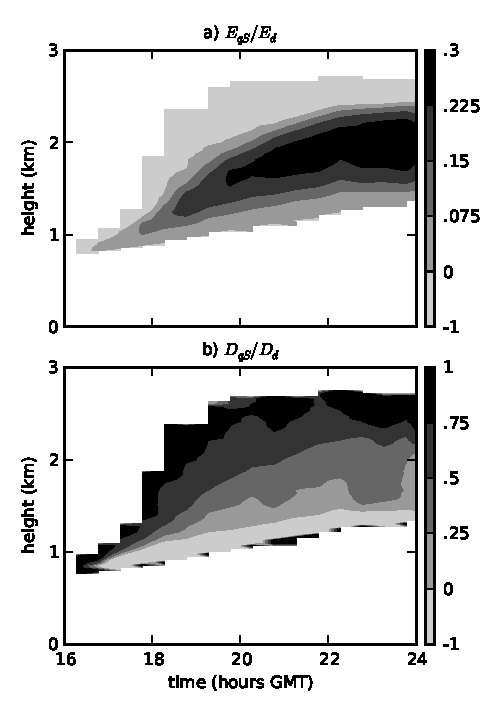
\includegraphics[width=19pc]{./figures/entrainment_ratio_variability}\\
  \caption{Variability of the ratio of the Siebesma tracer budget a) entrainment
  and b) detrainment values to the directly calculated values over the duration
  of the ARM model run.}
  \label{fig:entrainment_ratio_variability}
\end{figure}

\begin{figure}[t]
  \noindent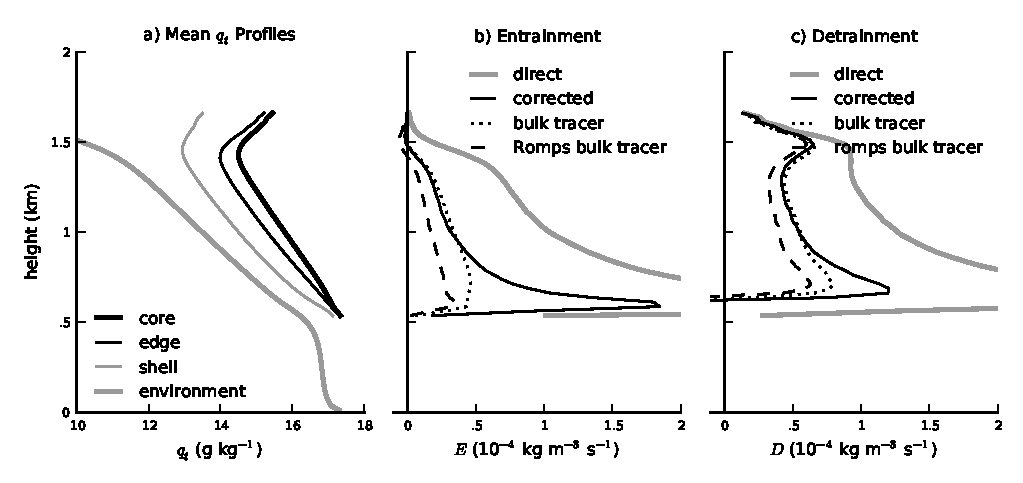
\includegraphics[width=39pc,angle=0]{./figures/shell_correction}\\
  \caption{Result of transforming direct entrainment values into equivalent 
  tracer budget values using mean cloud core shell and edge properties.  
  a) Mean profiles of the total specific humidity in the cloud core (thick 
  black line), cloud core edge (thin black line), cloud core shell (thin 
  grey line), and cloud core environment (thick grey line).  These $q_t$ 
  values are used to transform directly calculated values of b) entrainment 
  and c) detrainment (grey line) into equivalent tracer budget values 
  (black line).  The Siebesma tracer budget entrainment and detrainment
  are shown for comparison (dotted lines).}
  \label{fig:Shell_correction}
\end{figure}

\begin{figure}[t]
  \noindent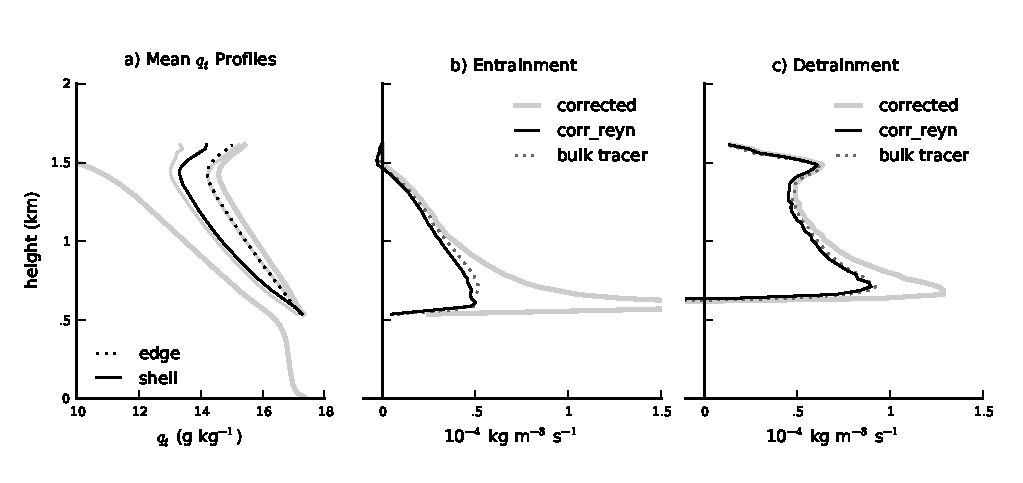
\includegraphics[width=39pc,angle=0]{./figures/reynolds_correction}\\
  \caption{Result of transforming direct entrainment values into equivalent 
  tracer budget values using effective entrainment and detrainment properties.
  a) Mean profiles of the effective total specific humidity values being
  entrained ($q_{entrain}$, black line), and detrained ($q_{detrain}$ dotted
  line), overlaid on the mean total specific humidity values of the core, edge, 
  shell and environment.  These $q_t$ values are used to transform directly 
  calculated values of b) entrainment and c) detrainment (grey line) into 
  equivalent tracer budget values (black line).  The Siebesma tracer 
  budget entrainment and detrainment are shown for comparison (dotted lines).}
  \label{fig:Reynolds_correction}
\end{figure}

\begin{figure}[t]
  \noindent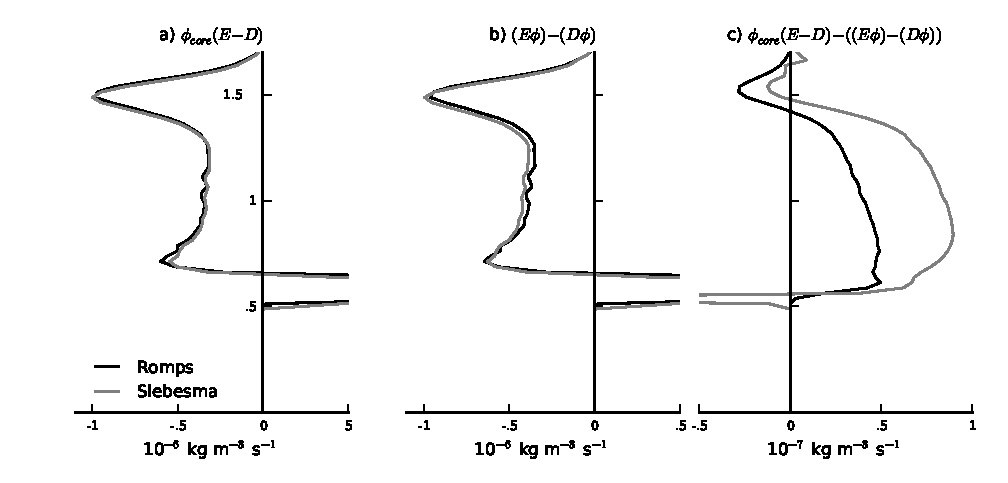
\includegraphics[width=39pc]{./figures/numerical_error}\\
  \caption{Size of a) $q_{core}(E-D)$, b) $Eq_t-Dq_t$ and c) the resulting 
  cloud core vertical advection and time tendency specific humidity budget 
  $VATT=q_{core}(E-D) - (Eq_t-Dq_t)$ for the direct entrainment/detrainment 
  (black lines), the direct entrainment/detrainment without time averaging 
  (grey lines), and the Siebesma tracer budget entrainment/detrainment 
  (dotted lines).}
  \label{fig:numerical_error}
\end{figure}

\begin{figure}[t]
  \noindent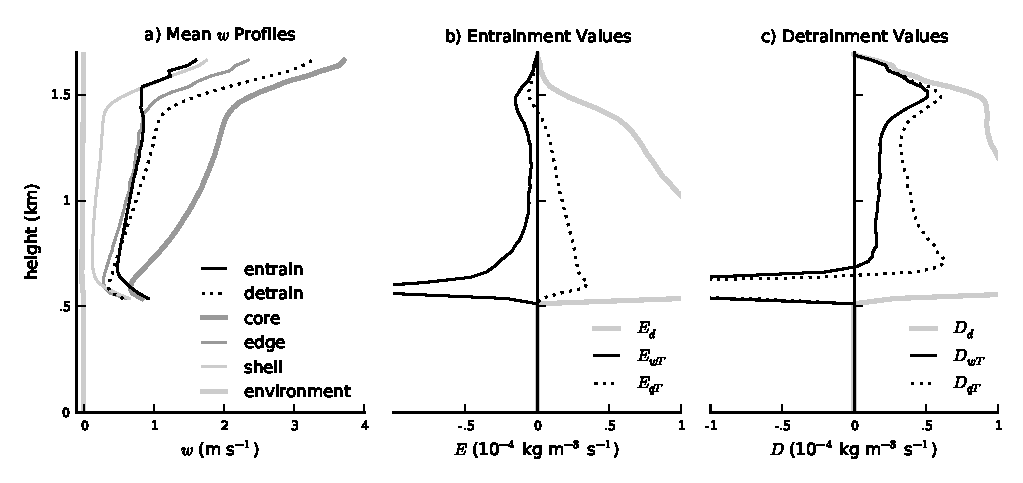
\includegraphics[width=39pc]{./figures/reynolds_correction_w}
  \caption{Result of transforming direct entrainment values into equivalent 
  $w$ budget values.  a) Mean profiles of the effective $w$ values being
  entrained (black line), and detrained (dotted line), overlaid on the mean 
  $w$ values of the core, edge, shell and environment.  These $w$ values are
  used to transform directly calculated values of b) entrainment and 
  c) detrainment (grey line) into equivalent tracer budget values (black 
  line).  The entrainment and detrainment values transformed using $q_t$ 
  are shown for comparison (dotted lines).}
  \label{fig:Reynolds_correction_w}
\end{figure}

\begin{figure}[t]
  \noindent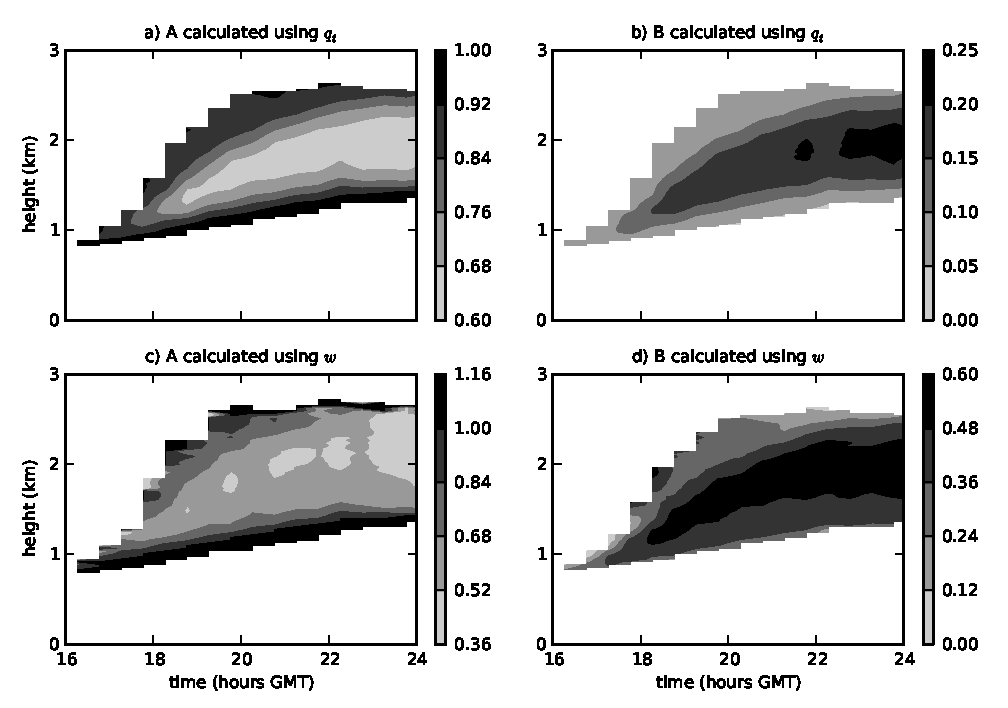
\includegraphics[width=39pc]{./figures/shell_variability}
  \caption{Variation in a) $(q_{entrain} - q_{env})/(q_{core} - q_{env})$,  
  b) $(q_{core} - q_{detrain})/(q_{core} - q_{env})$,  
  c) $(w_{entrain} - w_{env})/(w_{core} - w_{env})$, and 
  d) $(w_{core} - q_{detrain})/(w_{core} - w_{env})$ over the duration of the 
  ARM model run.
  }
  \label{fig:shell_variability}
\end{figure}

\begin{figure}[t]
  \noindent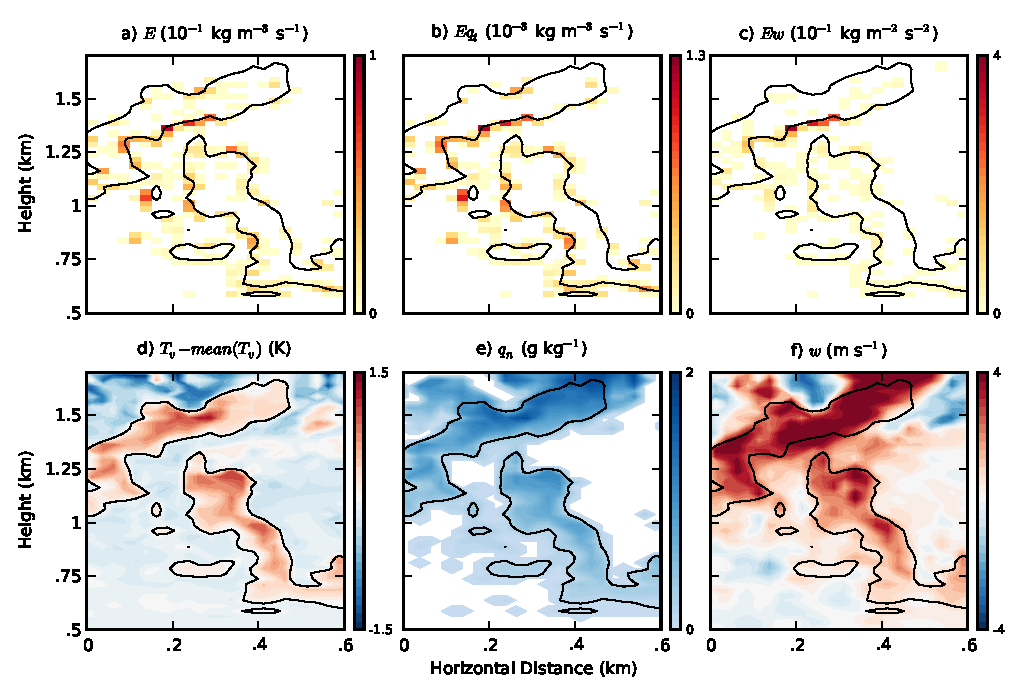
\includegraphics[width=39pc]{./figures/w_entrainment_example}
  \caption{Instantaneous vertical cross-section of directly calculated cloud 
  core mass entrainment (a), humidity entrainment (b), vertical velocity
  entrainment (c), buoyancy (d), condensed liquid water (e), and vertical
  velocity (f) of a single model cloud, illustrating the strong correlation
  between vertical velocity and entrainment.  Black lines indicate the edge of
  the cloud core in each figure.}
  \label{fig:w_entrainment_example}
\end{figure}

\end{document}
